% This must be in the first 5 lines to tell arXiv to use pdfLaTeX, which is strongly recommended.
\pdfoutput=1
% In particular, the hyperref package requires pdfLaTeX in order to break URLs across lines.

\documentclass[11pt]{article}

% Remove the "review" option to generate the final version.
\usepackage[review]{acl}

% Standard package includes
\usepackage{times}
\usepackage{latexsym}

% For proper rendering and hyphenation of words containing Latin characters (including in bib files)
\usepackage[T1]{fontenc}
% For Vietnamese characters
% \usepackage[T5]{fontenc}
% See https://www.latex-project.org/help/documentation/encguide.pdf for other character sets

% This assumes your files are encoded as UTF8
\usepackage[utf8]{inputenc}

\usepackage{graphicx}
\graphicspath{{images/}}

\usepackage{amsfonts}
\usepackage{amsmath}
\usepackage{amssymb}
\usepackage{amsthm}
\usepackage{bbm}


% This is not strictly necessary, and may be commented out,
% but it will improve the layout of the manuscript,
% and will typically save some space.
\usepackage{microtype}

\newtheorem{theorem}{Theorem}

% If the title and author information does not fit in the area allocated, uncomment the following
%
%\setlength\titlebox{<dim>}
%
% and set <dim> to something 5cm or larger.

\title{On the Evaluation of Neural Selective Prediction Methods for Natural Language Processing}

% Author information can be set in various styles:
% For several authors from the same institution:
% \author{Author 1 \and ... \and Author n \\
%         Address line \\ ... \\ Address line}
% if the names do not fit well on one line use
%         Author 1 \\ {\bf Author 2} \\ ... \\ {\bf Author n} \\
% For authors from different institutions:
% \author{Author 1 \\ Address line \\  ... \\ Address line
%         \And  ... \And
%         Author n \\ Address line \\ ... \\ Address line}
% To start a seperate ``row'' of authors use \AND, as in
% \author{Author 1 \\ Address line \\  ... \\ Address line
%         \AND
%         Author 2 \\ Address line \\ ... \\ Address line \And
%         Author 3 \\ Address line \\ ... \\ Address line}


\begin{document}
\maketitle
\begin{abstract}
We provide a survey and empirical comparison of the state-of-the-art in neural selective classification for NLP tasks. We also provide a methodological blueprint, including a novel metric called \emph{refinement} that provides a calibrated evaluation of confidence functions for selective prediction. Finally, we supply documented, open-source code to support the future development of selective prediction techniques. 
\end{abstract}

\section{Introduction}

Deep learning has brought massive improvements to natural language processing over the past decade, but neural networks still make mistakes. Accordingly, there is a current interest in confidence estimation techniques that perform well on deep neural networks. A prominent subarea of confidence estimation is \emph{selective prediction} \cite{el2010foundations,geifman2017selective}. Selective prediction focuses on developing classifiers that choose to abstain when sufficiently uncertain. There is less focus on absolute measures of confidence, and more on a classifier's ability to successful rank its predictions, enabling techniques that maximize prediction quality given a desired yield \cite{geifman2019selectivenet} or that maximize yield given a desired quality \cite{geifman2017selective}.  


This paper provides a survey and rigorous empirical comparison of the state-of-the-art in \emph{neural selective classification} (i.e. selective prediction where the underlying classifier is a neural network) specifically as it pertains to natural language processing. Our main contributions are the following:

\begin{itemize}
	\item We survey a variety of recent techniques proposed in the ML and NLP literature and compare them across \textbf{six} classification tasks from the \textsc{GLUE} benchmark \cite{wang-etal-2018-glue}. We do careful hyperparameter tuning for all surveyed techniques, and perform multiple trials of each technique to get an adequate sense of median and variance.
	\item Inspired by \cite{xin-etal-2021-art} and Kendall-tau distance \cite{kendall1948rank}, we propose a simple metric called \emph{refinement} that provides a calibrated measure of the performance of selective classification techniques.
	\item We determine that using maximum softmax probability as a confidence indicator remains a strong baseline, but Monte Carlo Dropout \cite{gal2016dropout} demonstrates significant improvement across multiple tasks and trials.
	\item We release a documented Python package called \textsf{spred} (\textbf{s}elective \textbf{pred}iction) to make our experiments transparent and reproducible. To facilitate evaluation of future techniques, the package provides tutorials about how to add and evaluate novel selective prediction methods.
\end{itemize}

\section{Selective Prediction}

\subsection{Preliminaries}

A \emph{prediction function} is a function $f: \mathcal{X} \rightarrow \mathcal{Y}$ that maps an instance space $\mathcal{X}$ to a label space $\mathcal{Y}$. We refer to the output $f(x)$ of the prediction function as its \emph{prediction} for instance $x \in \mathcal{X}$. We use the notation $\checkmark(x)$ to refer to the gold prediction for a particular instance. The following denotes the correctly and incorrectly predicted instances of prediction function $f$ on set $\mathbf{x} \subseteq \mathcal{X}$:
\begin{eqnarray*}
\mathcal{C}(f,\mathbf{x})
&= \{ x \in \mathbf{x} \mid f(x) = \checkmark(x) \} \\
\overline{\mathcal{C}}(f,\mathbf{x})
&= \{ x \in \mathbf{x} \mid f(x) \neq \checkmark(x) \}
\end{eqnarray*}


\noindent If we pair a prediction function with a \emph{selection function} $\tilde{g}: \mathcal{X} \rightarrow \{0,1\}$, we obtain a \emph{selective model} $(f,\tilde{g})$. For instance $x \in \mathcal{X}$, a selective model $h = (f, \tilde{g})$ \emph{publishes} its prediction $f(x)$ if $\tilde{g}(x)=1$, and \emph{abstains} if $\tilde{g}(x)=0$. In short:
\begin{gather*}
h(x) = \begin{cases}
               f(x) &\mbox{ if } \tilde{g}(x)=1\\
               \bot &\mbox{ if } \tilde{g}(x)=0
       \end{cases}
\end{gather*}

\noindent where $\bot$ is a symbol representing abstention. A convenient way to implement a selection function is to use a \emph{confidence function} $g: \mathcal{X} \rightarrow \mathbb{R}$ that assigns a real-valued confidence to any instance $x \in \mathcal{X}$. We can derive a selection function $\tilde{g}_\theta$ from confidence function $g$ by specifying a minimum confidence threshold $\theta \in \mathbb{R}$ for publishing predictions:

\begin{equation*}
\tilde{g}_\theta(x) = \mathbbm{1}[g(x) > \theta]
\end{equation*}

\subsection{Examples}

\begin{figure}
\centering
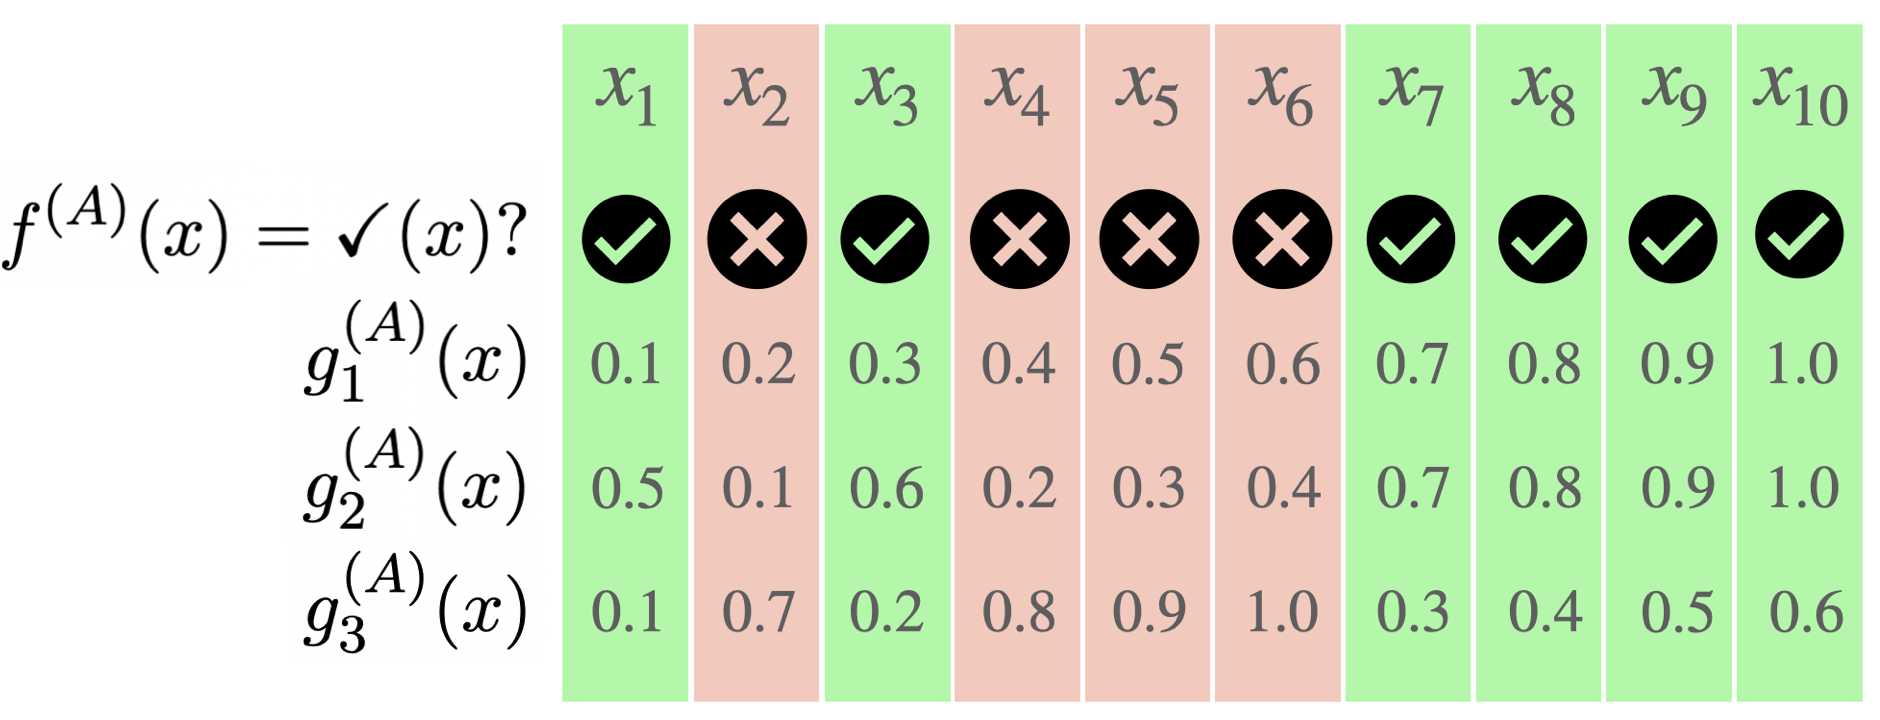
\includegraphics[width=0.48\textwidth]{example1.png}
\caption{Three confidence functions for an example prediction function that has an overall accuracy of 6/10 on the evaluation set.}
\label{fig:example1}
\end{figure}

\begin{figure}
\centering
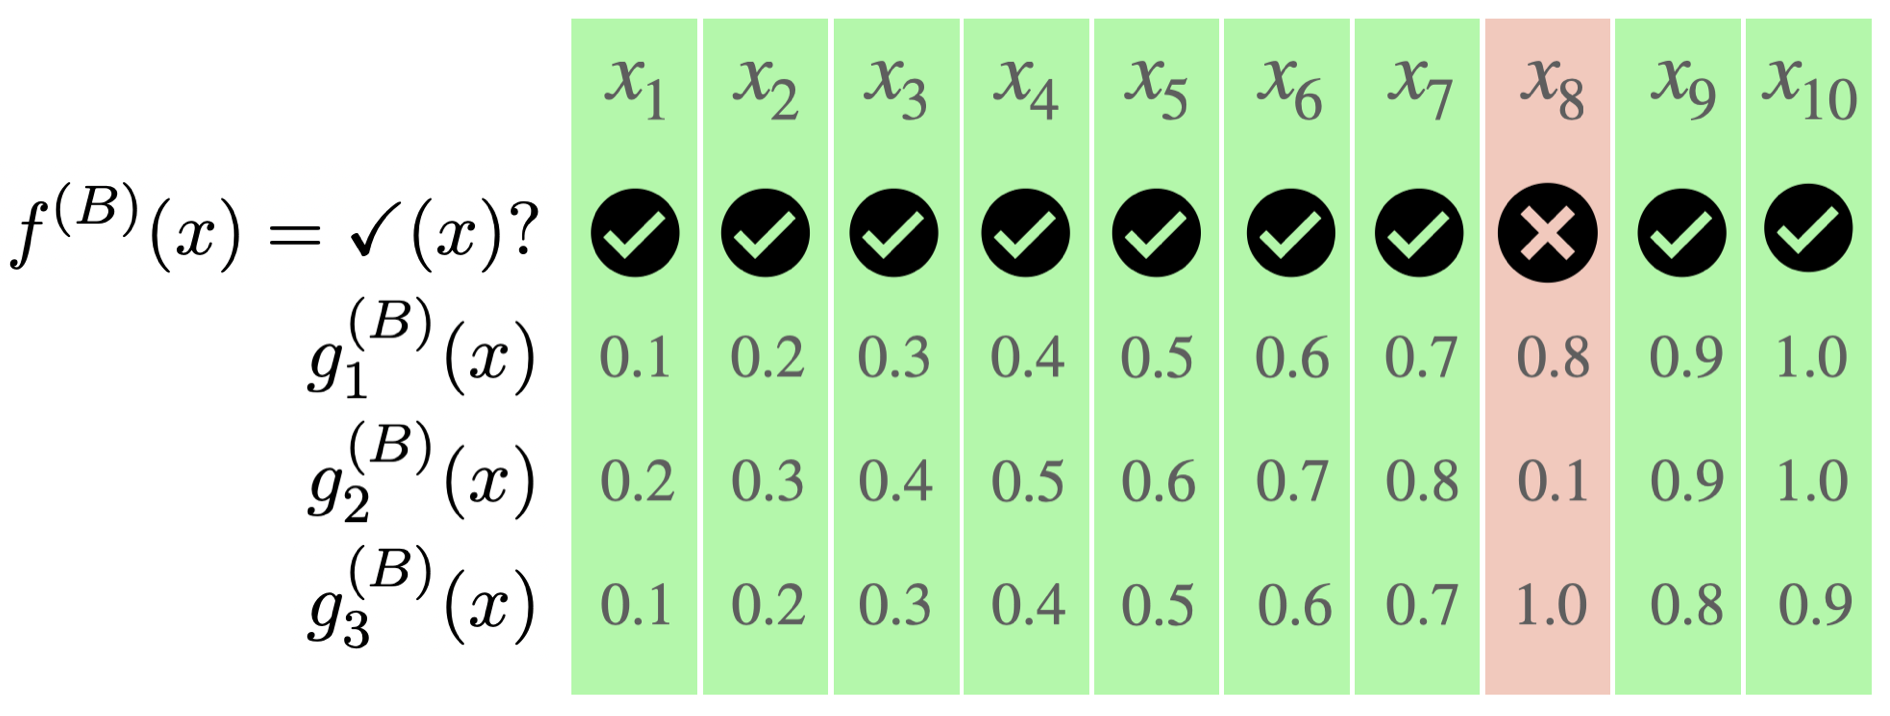
\includegraphics[width=0.48\textwidth]{example2.png}
\caption{Three confidence functions for a stronger prediction function that has an overall accuracy of 9/10 on the evaluation set.}
\label{fig:example2}
\end{figure}


In Figure~\ref{fig:example1}, we show three confidence functions $g_1^{(A)}$, $g_2^{(A)}$, $g_3^{(A)}$ for an example prediction function $f^{(A)}$. The first confidence function $g_1^{(A)}$ is pretty good; it assigns its highest confidences to four out of the six correct predictions, though unfortunately it also gives its lowest confidence to the correct prediction $f^{(A)}(x_1)$. The superior $g_2^{(A)}$ is a best-case confidence function (assigning its highest confidences to the six correct predictions) and $g_3^{(A)}$ is a worst-case confidence function (assigning its lowest confidences to the six correct predictions).

Figure~\ref{fig:example2} shows three more confidence functions $g_1^{(B)}$, $g_2^{(B)}$, $g_3^{(B)}$ for a stronger prediction function $f^{(B)}$. This time, the first confidence function $g_1^{(B)}$ is not particularly good; it assigns its third-highest confidence to the only incorrect prediction. Again, $g_2^{(B)}$ is a best-case confidence function (assigning its highest confidences to the nine correct predictions) and $g_3^{(B)}$ is a worst-case confidence function (assigning its lowest confidences to the nine correct predictions). 

\begin{figure*}[t]
\centering
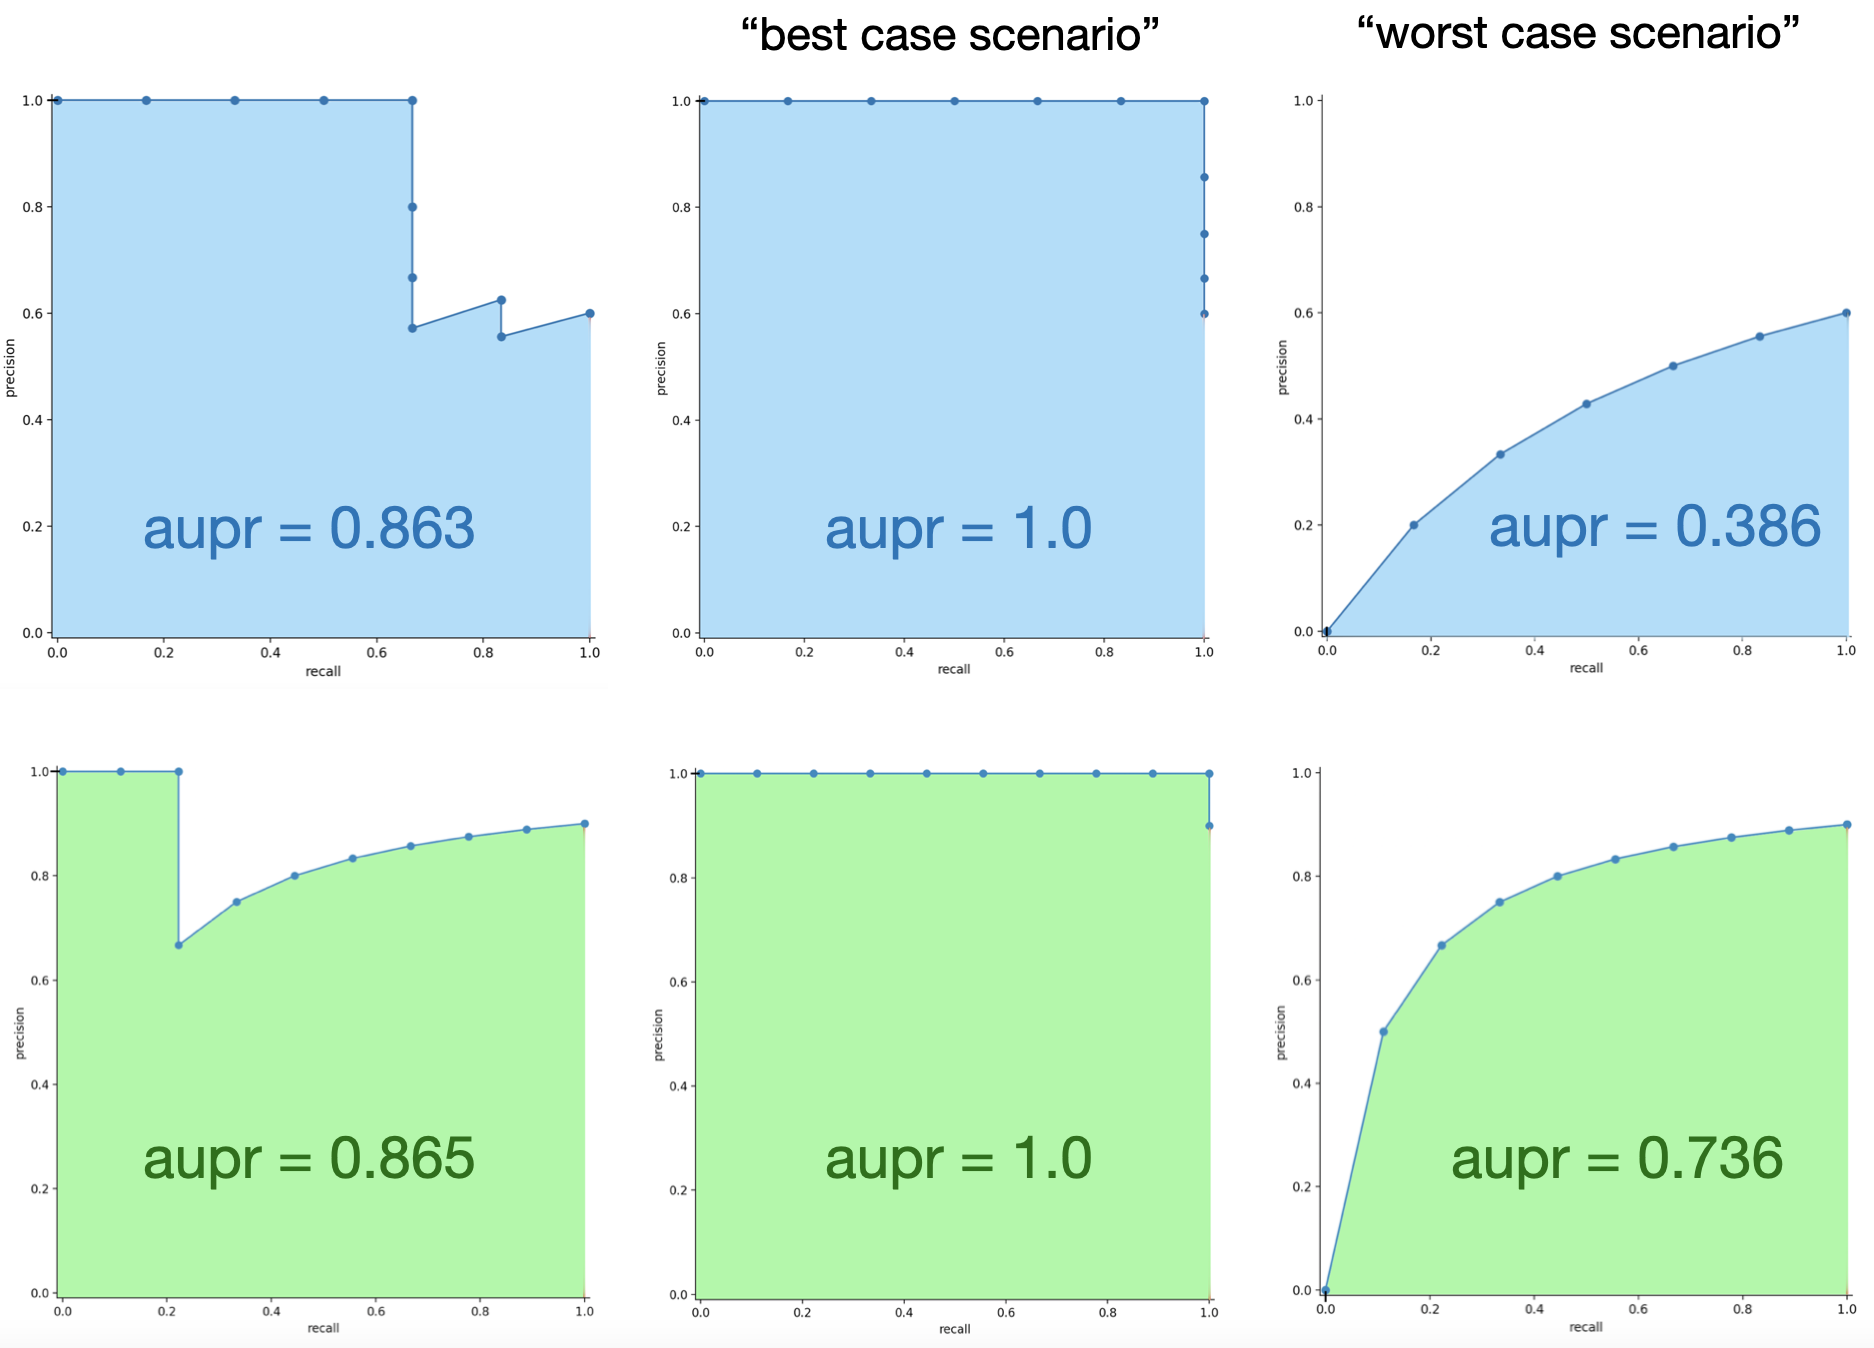
\includegraphics[width=0.88\textwidth]{pr_curves.png}
\caption{Precision-recall curves for confidence functions $g_1^{(A)}$, $g_2^{(A)}$, $g_3^{(A)}$ (top, blue) and confidence functions $g_1^{(B)}$, $g_2^{(B)}$, $g_3^{(B)}$ (bottom, green).}
\label{fig:pr_curves}
\end{figure*}


\subsection{Evaluation with AUC Metrics}

Typically, one evaluates the goodness of a confidence function by quantifying the trade-off between the quality and quantity of its published predictions. Since the prominent approaches -- risk/coverage curves \cite{el2010foundations}, receiver-operator (ROC) curves \cite{Davis06}, and precision-recall curves \cite{HendrycksG17} -- share many of the same benefits and drawbacks (some of which we discuss in this section), we will focus on precision-recall curves, mainly due to the NLP community's increased familiarity with them. In Figure~\ref{fig:pr_curves}, we show the precision-recall curves for the six confidence functions from the previous subsection. The aspiration of any confidence function is to achieve an \textbf{A}rea \textbf{U}nder the \textbf{P}recision-\textbf{R}ecall curve (AUPR) of 1, which means that it has perfectly separated the correct and incorrect predictions of the prediction function. Among the examples, this has been achieved by confidence functions $g_2^{(A)}$ and $g_2^{(B)}$.

A drawback with AUPR (and its analogs) is that its value is not interpretable without knowledge of the goodness of the associated prediction function. To see why, suppose we replace confidence function $g_1^{(A)}$ with a random confidence function $g_\mathsf{rnd}$, i.e. we choose each confidence $g_\mathsf{rnd}(x)$ uniformly at random from the interval $(0,1)$. Empirically, we observe an average AUPR\footnote{Averaged over 200 random confidence functions.} of approximately 0.64 for a random confidence function $g_\mathsf{rnd}$ associated with prediction function $f^{(A)}$. Since this is considerably worse than the AUPR (0.863) of confidence function $g_1^{(A)}$, we can surmise that confidence function $g_1^{(A)}$ is ``better than random''. By contrast, a random confidence function associated with the superior prediction function $f^{(B)}$ yields a empirical average AUPR\footnote{Again, averaged over 200 random confidence functions.} of approximately 0.91, which is considerably \textbf{better} than the AUPR (0.865) of confidence function $g_1^{(B)}$ -- thus confidence function $g_1^{(B)}$ is ``worse than random''.

Both $g_1^{(A)}$ and $g_1^{(B)}$ have AUPRs of approximately 0.86, but the former is ``better than random," while the latter is ``worse than random." Thus, AUPR does not provide a standalone indicator of the quality of a confidence function. This is because AUPR is a composite of the goodness of the confidence function and the goodness of the prediction function. One could imagine calibrating AUPR by taking into account the worst-case AUPR (i.e. the AUPRs for worst-case confidence functions $g_3^{(A)}$ and $g_3^{(B)}$) but we will adopt an even simpler approach based on a recent proposal by \cite{xin-etal-2021-art}.

\subsection{Evaluation with Kendall-tau Distance}

\begin{figure}[t]
\centering
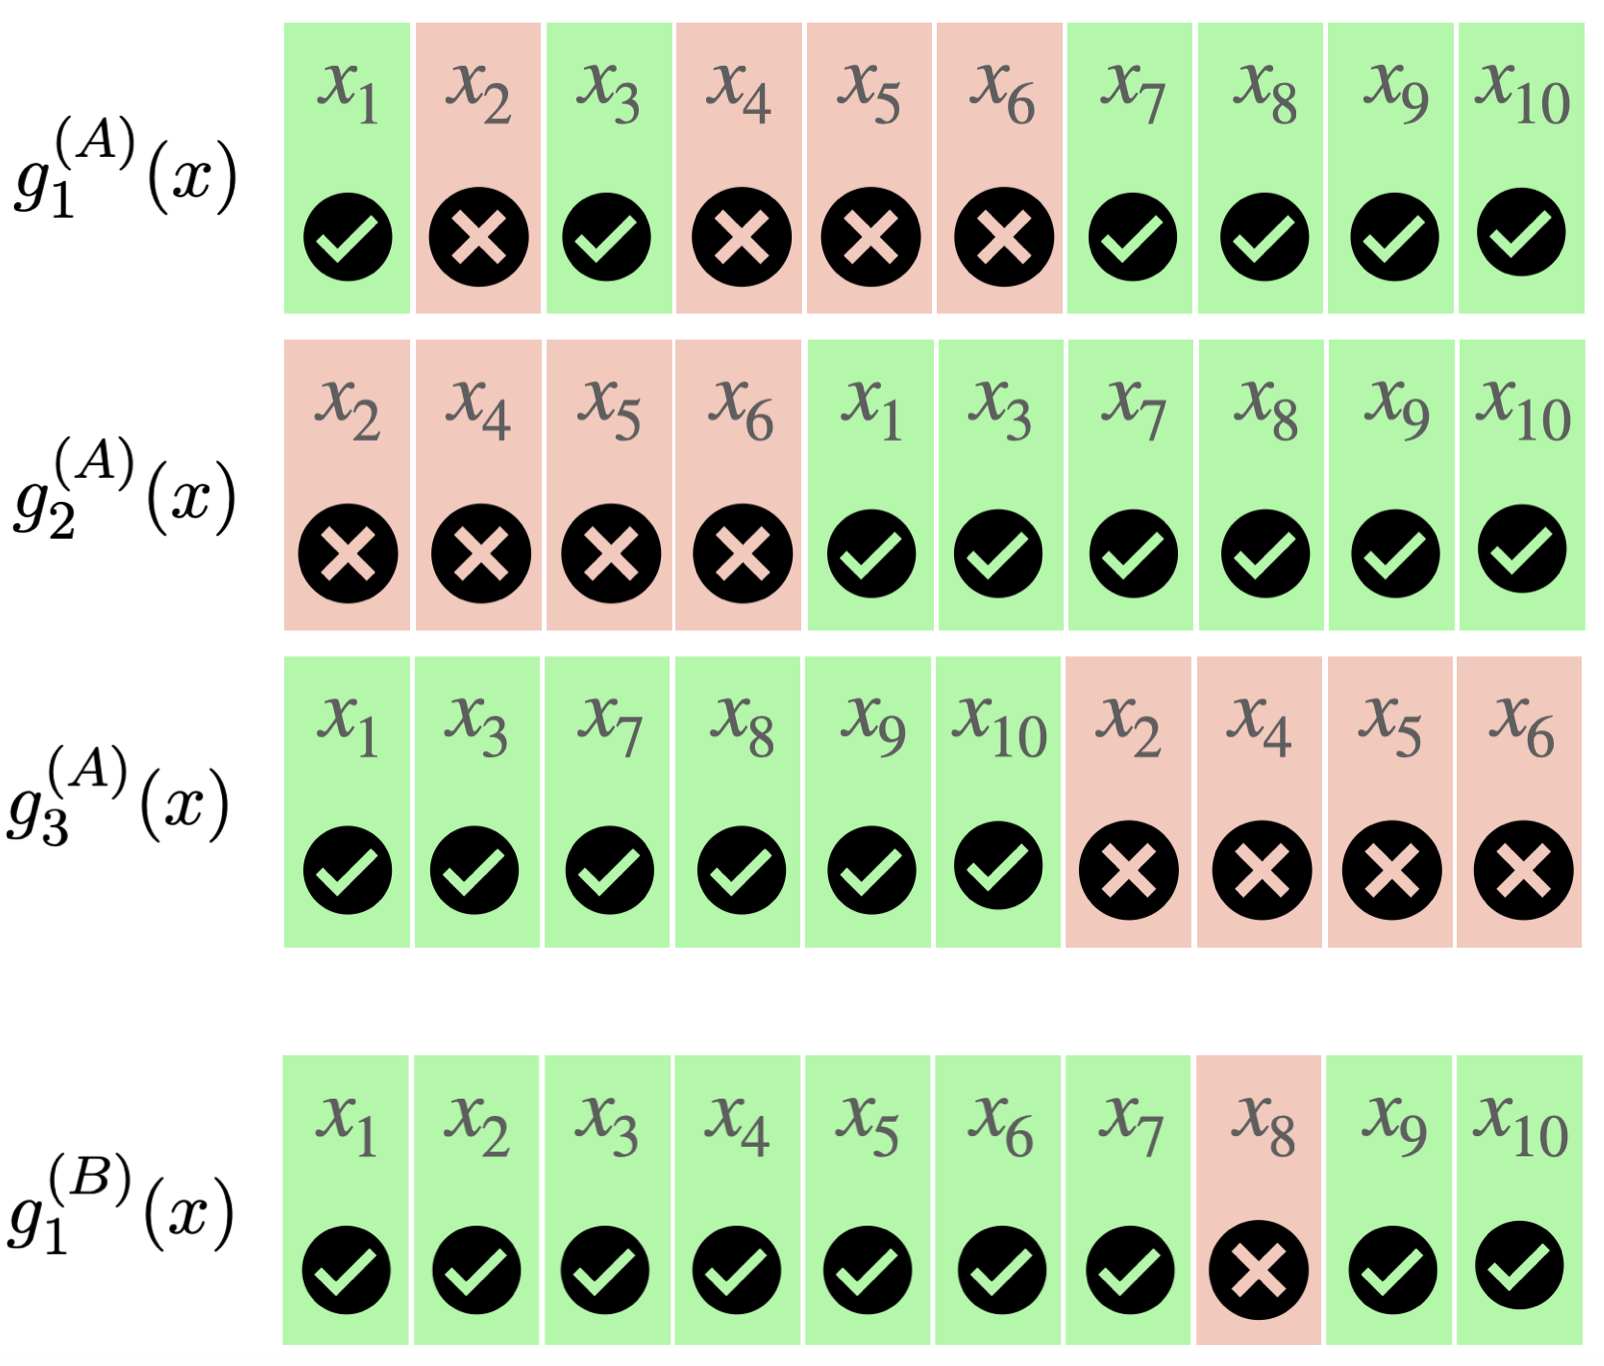
\includegraphics[width=0.48\textwidth]{rankedall.png}
\caption{The predictions of four of our example confidence functions, sorted by increasing confidence. The RPP for $g_1^{(A)}$ and $g_1^{(B)}$ are equivalent, although the former is better than random and the latter is worse than random.}
\label{fig:ranked}
\end{figure}


If we sort predictions by increasing confidence (as in Figure~\ref{fig:ranked}), a best-case confidence function (e.g. $g_2^{(A)}$) ranks all incorrect predictions below all correct predictions, while a worst-case confidence function (e.g. $g_3^{(A)}$) ranks all \emph{correct} predictions below all \emph{incorrect} predictions. Observing this, \cite{xin-etal-2021-art} proposed a rank-based evaluation metric for selective prediction called \textbf{R}eversed \textbf{P}air \textbf{P}roportion (RPP), which is a normalized count of pairwise ranking errors, i.e. a normalized version of Kendall-tau distance \cite{kendall1948rank}: 
\begin{eqnarray*}
\tau_{f, \mathbf{x}}(g) &=& \sum_{\substack{
x_{\textcolor{olive}{\checkmark}} \in \mathcal{C}(f, \mathbf{x})\\
x_{\textcolor{red}{\times}} \in \overline{\mathcal{C}}(f, \mathbf{x})}} \mathbbm{1}[g(x_{\textcolor{olive}{\checkmark}}) < g(x_{\textcolor{red}{\times}})] \\
\textsc{RPP}_{f, \mathbf{x}}(g) &=& \frac{\tau_{f, \mathbf{x}}(g)}{|\mathbf{x}|^2}
\end{eqnarray*}
For instance, confidence function $g_1^{(A)}$ has a Kendall-tau distance of 7 (it misranks correct instance $x_1$ below 4 incorrect predictions, and instance $x_3$ below 3 incorrect predictions) and an RPP of $\frac{7}{100}$. For the best-case confidence function $g_2^{(A)}$, $\tau_{f, \mathbf{x}}(g_2^{(A)}) = \textsc{RPP}_{f, \mathbf{x}}(g_2^{(A)}) = 0$. Unfortunately, using $|\mathbf{x}|^2$ as the normalizer means that RPP suffers the same issue as AUPR: its value cannot be interpreted independently of the goodness of the prediction function. Consider the RPP for our ``worse-than-random'' confidence function $g_1^{(B)}$. Like $g_1^{(A)}$, it has a Kendall-tau distance of 7 (it misranks incorrect instance $x_8$ above 7 correct predictions) and thus an RPP of $\frac{7}{100}$. Even though $g_1^{(A)}$ is better than random and $g_1^{(B)}$ is worse than random, they end up with the same RPP. 

%\begin{figure}
%\centering
%\includegraphics[width=0.48\textwidth]{ranked2.png}
%\caption{The predictions of $g_1^{(B)}$, sorted by increasing confidence. Both $\tau_{dist}$ and RPP for $g_1^{(A)}$ and $g_1^{(B)}$ are equivalent.}
%\label{fig:ranked2}
%\end{figure}

Fortunately, there is a simple remedy: all we need to do is normalize by the worst-case Kendall-tau distance $c(|\mathbf{x}|-c)$, where $c$ is the number of correct predictions made by the prediction function. To obtain a metric with a similar interpretation to accuracy and AUPR (for which higher values are ``better''), we subtract this new normalized distance from one, resulting in a measurement we call \emph{refinement}:

\begin{equation*}
\mathcal{R}_{f, \mathbf{x}}(g) = 1 - \frac{\tau_{f, \mathbf{x}}(g)}{c(|\mathbf{x}|-c)}
\end{equation*}

\noindent where $c = |\mathcal{C}(f, \mathbf{x})|$. Refinement has the following appealing properties:

\begin{theorem}
	If $0 < |\mathcal{C}(f, \mathbf{x})| < |\mathbf{x}|$ (i.e. prediction function $f$ makes at least one correct prediction and at least one incorrect prediction), then:
	\begin{gather*}
		\min_{g} \mathcal{R}_{f, \mathbf{x}}(g) = 0\\
		\max_{g} \mathcal{R}_{f, \mathbf{x}}(g) = 1
	\end{gather*}
\end{theorem}

\begin{proof}
	Consider prediction function $f$ and instance set $\mathbf{x}$ such that $0 < |\mathcal{C}(f, \mathbf{x})| < |\mathbf{x}|$, which implies that $c(|\mathbf{x}|-c) > 0$. Since $0 \leq \tau_{f, \mathbf{x}}(g) \leq c(|\mathbf{x}|-c)$, therefore $0 \leq \mathcal{R}_{f, \mathbf{x}}(g) \leq 1$. To prove the theorem, then, we need only show these bounds are tight, i.e. construct two confidence functions $g_\mathsf{min}(x)$ and  $g_\mathsf{max}(x)$ such that $g_\mathsf{min}(x) = 0$ and $g_\mathsf{max}(x) = 1$. Let:
	\begin{gather*}
	g_\mathsf{min}(x) = \begin{cases}
               0.4 &\mbox{ if } x \in \mathcal{C}(f, \mathbf{x})\\
               0.6 &\mbox{ if } x \in \bar{\mathcal{C}}(f, \mathbf{x})
       \end{cases}\\
	g_\mathsf{max}(x) = \begin{cases}
               0.4 &\mbox{ if } x \in \bar{\mathcal{C}}(f, \mathbf{x})\\
               0.6 &\mbox{ if } x \in  \mathcal{C}(f, \mathbf{x})
                   \end{cases}
	\end{gather*}
	 Then $\mathcal{R}_{f, \mathbf{x}}(g_\mathsf{min}) = 1-\frac{(|\mathbf{x}|-c)}{c(|\mathbf{x}|-c)} = 0$, and $\mathcal{R}_{f, \mathbf{x}}(g_\mathsf{max}) = 1-\frac{0}{c(|\mathbf{x}|-c)} = 1$. 
\end{proof}

\noindent In other words, a best-case confidence function has a refinement of 1, whereas a worst-case confidence function has a refinement of 0. Moreover:

\begin{theorem}
	For a random confidence function $g$, the expected value of $\mathcal{R}_{f, \mathbf{x}}(g)$ is 0.5.
\label{thm:expected}
\end{theorem}

\begin{proof}
Define binary random variable $Z_{ij}$ such that $Z_{ij}=1$ iff $g(x_i) < g(x_j)$. According to the definition of Kendall-tau distance:
\begin{equation*}
	\tau_{f, \mathbf{x}}(g) = \sum_{\substack{
x_i \in \mathcal{C}(f, \mathbf{x})\\
x_j \in \overline{\mathcal{C}}(f, \mathbf{x})}} Z_{ij}
\end{equation*}
By linearity of expectation:
\begin{eqnarray*}
	E(\tau_{f, \mathbf{x}}(g)) &=& E\left(\sum_{\substack{
x_i \in \mathcal{C}(f, \mathbf{x})\\
x_j \in \overline{\mathcal{C}}(f, \mathbf{x})}} Z_{ij}\right)\\
&=& \sum_{\substack{
x_i \in \mathcal{C}(f, \mathbf{x})\\
x_j \in \overline{\mathcal{C}}(f, \mathbf{x})}} E( Z_{ij} )\\
&=& \sum_{\substack{
x_i \in \mathcal{C}(f, \mathbf{x})\\
x_j \in \overline{\mathcal{C}}(f, \mathbf{x})}} 0.5\\
&=& 0.5 c(|\mathbf{x}|-c)
\end{eqnarray*}

\noindent And therefore:
\begin{eqnarray*}
	E(\mathcal{R}_{f, \mathbf{x}}(g)) &=& 
	1 - \frac{E(\tau_{f, \mathbf{x}}(g))}{c(|\mathbf{x}|-c)}\\
	&=& 1 - \frac{0.5 c(|\mathbf{x}|-c)}{c(|\mathbf{x}|-c)}\\
	&=& 0.5	
\end{eqnarray*}

\end{proof}



\noindent Unlike RPP and the various area under the curve metrics, refinement directly assesses the quality of the confidence function, and its value is calibrated and interpretable (0 = worst case, 0.5 = random confidence, 1.0 = best case) without knowledge of the quality of the associated prediction function.

\section{Surveyed Techniques}

Our main goal in this paper is a reproducible and thorough comparison of a broad range of selective prediction techniques on NLP tasks. In this section, we describe the techniques we compare. 

\subsection{Confidence Functions}

The following are ways to create a confidence function for an already trained neural prediction function.

\subsubsection*{\textsc{MaxProb}}

For neural prediction functions, the simplest-to-implement confidence function is likely \textsc{MaxProb}, shown here applied a three-way sentiment analysis task:
\begin{figure}[h]
\centering
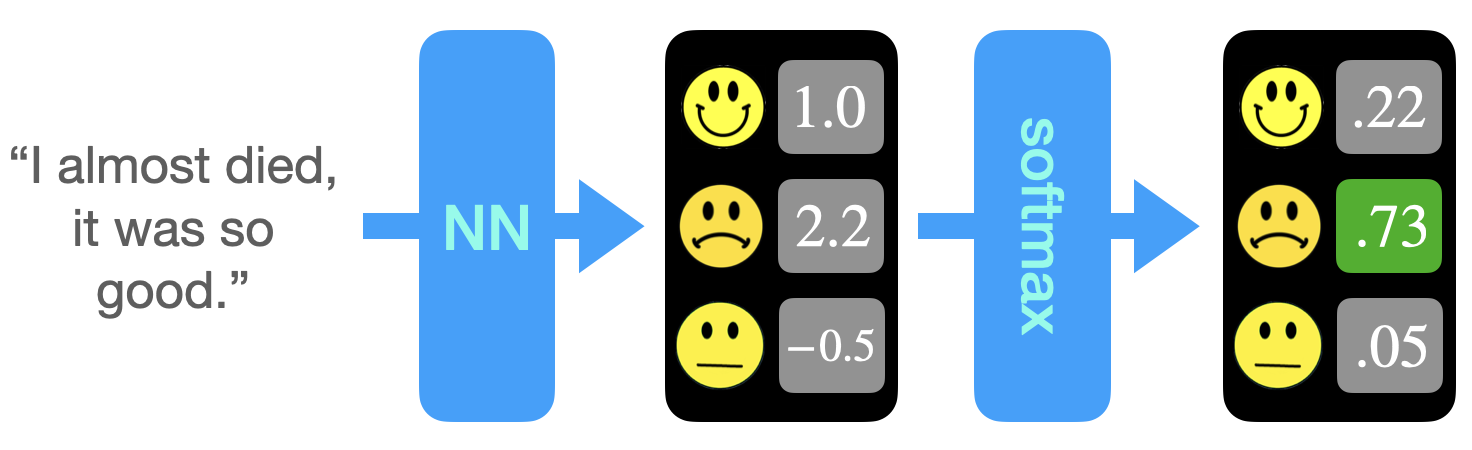
\includegraphics[width=0.48\textwidth]{softmax.png}
\label{fig:softmax}
\vspace{-10pt}
\end{figure}

\noindent After applying softmax to the neural network output, \textsc{MaxProb} (sometimes known as \textsc{SoftmaxResponse}) uses the maximum probability of the resulting distribution as its measure of confidence. The surprising effectiveness of such a simple approach was observed by \cite{HendrycksG17}, among others.

\subsubsection*{Monte Carlo Dropout (\textsc{McdM/McdV})}

\cite{gal2016dropout} proposed leveraging dropout \cite{srivastava2014} to assess the uncertainty of a neural network on a particular instance. As usual, dropout is disabled at test time to make the prediction. But then the input instance is re-decoded $k$ times with dropout enabled. This yields $k$ samples for the softmax probability of the prediction. There are two common methods \cite{kamath-etal-2020-selective} for synthesizing these $k$ samples into a confidence measure: either we take the mean \cite{lakshminarayanan2017simple} of the samples (a strategy we refer to as \textsc{McdM}), or the negative\footnote{We use the \emph{negative} variance  so that a greater value indicates a greater confidence.} variance \cite{feinman2017detecting,SmithG18} of the samples (a strategy we refer to as \textsc{McdV}).


\subsubsection*{\textsc{TrustScore}}

\cite{jiang2018trust} advocated a nearest-neighbor-based confidence function. First, the training instances are converted\footnote{They are agnostic about how best to do so. We will return to this issue.} into vector encodings, and grouped according to their gold labels. Outliers are then filtered from each labeled group. Specifically, they sort the vectors (i.e. points in $\mathbb{R}^d$ space) by the radius of the minimal ball centered at that vector that contains $k$ points from their labeled group. The percentage $\alpha \in [0, 1]$ of points with the largest such radii (i.e. the outliers) are removed. This filtered set\footnote{They fix $k=10$, but treat $\alpha$ as a tunable hyperparameter.} is called an $\alpha$-\emph{high density set}. The confidence assigned to an instance prediction, called \textsc{TrustScore}, is the ratio of (a) the distance between the instance's vector encoding and the closest $\alpha$-high density set of a \emph{non-predicted} label, (b) the distance between the instance's vector encoding and the $\alpha$-high density set of the \emph{predicted} label.

\subsection{Specialized Loss Functions}

We also survey techniques that simultaneously train a prediction function and an associated confidence function. 

\subsubsection*{Error Regularization (\textsc{EReg})}

\cite{xin-etal-2021-art} suggests adding an ``error regularization" term to the task's loss function $\mathcal{L}$ that directly penalizes ranking errors made by the confidence function $g$:
\begin{gather*}
\epsilon(f, \mathbf{x}) = \sum_{\substack{
x_{\textcolor{olive}{\checkmark}} \in \mathcal{C}(f, \mathbf{x})\\
x_{\textcolor{red}{\times}} \in \overline{\mathcal{C}}(f, \mathbf{x})}} \bigl[ \max(0, g(x_{\textcolor{red}{\times}}) - g(x_{\textcolor{olive}{\checkmark}})) \bigr] ^2 \\
\mathcal{L}_{\textsc{EReg}}(f, \mathbf{x}) = \mathcal{L}(f, \mathbf{x}) + \lambda \cdot \sum_{\mathbf{b} \in \mathsf{batches}(\mathbf{x})} \epsilon(f, \mathbf{b})
\end{gather*}

\noindent where $\lambda \in \mathbb{R}^+$ is a tunable hyperparameter and $\mathsf{batches}(\mathbf{x})$ is the set of minibatches of training set $\mathbf{x}$. At training time, \cite{xin-etal-2021-art} uses \textsc{MaxProb} for the confidence function $g$, though at test time, they additionally experiment with \textsc{McdM} and \textsc{McdV}.


\subsubsection*{Deep Abstaining Classifiers (\textsc{DAC})}


A Deep Abstaining Classifier \cite{thulasidasan2019combating}, abbreviated DAC, explicitly introduces an extra abstention output $\bot$ to the neural network, and trains with a loss function that allows the prediction function to benefit from abstaining on difficult instances:
\begin{equation*}
	\mathcal{L}_{\textsc{DAC}}(f, \mathbf{x}) = (1-p_\bot) \mathcal{L}(f, \mathbf{x}) + \alpha \log \frac{1}{1-p_\bot}
\end{equation*}

\noindent where $p_\bot$ is the probability according to abstention output $\bot$ after applying softmax, $\mathcal{L}(f, \mathbf{x})$ is standard cross-entropy loss over the non-abstention outputs, and $\alpha$ is a real-valued weight that is zero for the first $k$ (warmup) epochs of training, and is linearly scaled from $\alpha_{min}$ to $\alpha_{max}$ during the remaining epochs. The initial value $\alpha_{min}$ is set to be a fixed fraction $\frac{1}{\rho}$ of a moving average of the loss during the warmup epochs. The authors provide code that we use in our experiments. At test time, \textsc{MaxProb} is used\footnote{We also experimented with using $1-p_\bot$ (i.e. the total probability mass accorded to non-abstention outputs) as the confidence, but this yielded poor results.} as the confidence function, though with a slight modification -- if the probability associated with the abstention label is the maximum softmax probability, then the next highest probability is used as the confidence.

\section{Experiment Design}
\label{sec:expdesign}


To draw reliable conclusions on a sufficiently varied set of NLP tasks, we evaluated the techniques on six classification\footnote{We did not include \textsc{wnli} because the training set was too small to train a prediction function that does better than random guessing. We did not include \textsc{qqp} because we had training difficulties that we could not resolve before the submission deadline. \textsc{sts-b} is a regression task, not a classification task. For evaluating \textsc{mnli}, we used matched accuracy, since the focus of this paper is not on domain shift.} tasks of the \textsc{GLUE} benchmark \cite{wang-etal-2018-glue}: \textsc{cola}, \textsc{mnli}, \textsc{mrpc}, \textsc{qnli}, \textsc{rte}, and \textsc{sst-2}. Bearing in mind that our goal is to compare selective classification techniques, not to produce state-of-the-art prediction functions, we randomly partitioned each training set into two halves, using \textsc{GlueTrain-A} for training and \textsc{GlueTrain-B} for early stopping and hyperparameter tuning. Since the gold labels for GLUE test sets are not all publicly available, we reserved the development set (\textsc{GlueDev}) of each task for final evaluation. We trained the prediction function by fine-tuning \textsc{bert-base-cased} using the \texttt{transformers} package \cite{wolf-etal-2020-transformers}, mostly using the training parameters recommended by its \texttt{run\_glue.py} script (the sole deviation is that we run each training for 6 epochs, rather than 3). For the techniques that required specialized loss functions, we substituted the default \textsc{BERT} loss function with the alternative specified by the selective prediction technique. 

\subsection{Hyperparameter Tuning}

In an effort to fairly evaluate each technique, we began with smaller-scale experiments to determine an appropriate setting of a technique's hyperparameters for the \textsc{GLUE} tasks. For these experiments, we used \textsc{GlueTrain-A} for training and \textsc{GlueTrain-B} for validation. We selected three \textsc{GLUE} tasks of various sizes and genres (one single-sentence task, one similarity-and-paraphrase task, and one inference task) as proxies: \textsc{sst-2}, \textsc{mrpc}, and \textsc{rte}. We ran 5 trials for each hyperparameter setting.

\subsubsection*{\textsc{McdM/McdV}}

The Monte Carlo Dropout techniques each have a single hyperparameter $k$: the number of decodings of the training instance with dropout enabled. We experimented with $k \in \{10, 30, 50\}$. We found little discernible difference (see Figure~\ref{fig:mcd_hparams}) between $k=30$ and $k=50$. Slightly better results with $k=30$ versus $k=10$ convinced us to use $k=30$ for further experiments.


\subsubsection*{\textsc{TrustScore}}

To use \textsc{TrustScore}, we need to encode each instance as a vector. Following common practice, we used BERT's final layer encoding (after finetuning) of the \textsc{[cls]} token. To select the hyperparameter settings for \textsc{TrustScore}, we followed \cite{jiang2018trust} and experimented with several powers of two for hyperparameter $\alpha$, specifically $\alpha \in \{0.5, 0.25, 0.125\}$. Also, since \textsc{TrustScore} is too slow in practice to run on large training sets, we sample $N$ training instances (without replacement) prior to running the TrustScore algorithm. In our tuning experiments, we tried the values $N \in \{800, 1600\}$. We found little difference between the six hyperparameter settings (see Figure~\ref{fig:ts_hparams}) and set $N=800$ and $\alpha=0.25$ for further experiments.

\subsubsection*{\textsc{EReg}}

\textsc{EReg} has hyperparameter $\lambda$ (the multiplier for the regularization term). Following the appendix of \cite{xin-etal-2021-art}, we experimented with $\lambda \in \{0.01, 0.05, 0.1, 0.5\}$. Because \textsc{EReg} uses an alternative loss function that can potentially affect the overall quality of the prediction function, we used AUPR (which blends the quality of the prediction function with the quality of the selection function) as our main evaluation metric. We found high variance between trials, and selected $\lambda = 0.05$ (with the most consistent performance) for further experiments. \textsc{EReg} is also affected by the minibatch size. If the minibatch size is 1, then the loss function reduces to the base loss function for the task. Larger minibatches increase the number of pairwise comparisons incorporated into the regularization term. For the final experiments (Section~\ref{sec:results}), we used\footnote{Unfortunately, many GPU machines (including the machine running our experiments) do not have sufficient memory to finetune PTLMs with larger batch sizes.} minibatch sizes of 8 and 16.

\subsubsection*{\textsc{DAC}}

One of the virtues of \textsc{DAC} is that it automatically adjusts its weights according to the cross-entropy loss observed during the warmup epochs, but it still has hyperparameters $\rho$ and $\alpha_{max}$ to determine precisely how this is done. In the code accompanying \cite{thulasidasan2019combating}, the default settings are $\rho=64$ and $\alpha_{max}=1.0$. Given these defaults, we experimented with $\rho \in \{32,64,128\}$ and $\alpha_{max}\in \{0.5, 1.0, 2.0\}$. The technique did not appear to be particularly sensitive to the choice of hyperparameters (see Figure~\ref{fig:dac_hparams}) and so we kept the default settings for further experiments. We used two warmup epochs (sufficient to reach decent baseline accuracy for all GLUE tasks), and accordingly increased the total number of training epochs from 6 to 8.


\section{Results}
\label{sec:results}


For final evaluation, we ran ten experiment trials on the six GLUE tasks. Specifically, we trained ten prediction functions with different random seeds for each loss function: the basic \textsc{bert} loss (\texttt{basic}), \textsc{bert} loss with error regularization (\texttt{ereg.b}, where $\texttt{b} \in \{8, 16\}$ is the minibatch size), and the Deep Abstaining Classifier loss (\texttt{dac}). For each resulting prediction function, we evaluated the various confidence functions. In all experiment trials, we used the hyperparameter settings established in Section~\ref{sec:expdesign}. Figure~\ref{fig:posthocviolin} visualizes the results\footnote{For visual clarity, we omit certain loss/confidence pairs from Figure~\ref{fig:posthocviolin}, for instance \texttt{ereg(mcdm)} and \texttt{ereg(mcdv)}. In our experiments, the MC Dropout techniques provided similar improvement for all loss functions.} for two GLUE datasets (\textsc{mrpc} and \textsc{sst-2}) using a violin plot\footnote{We used the \texttt{seaborn} package to create the plots: \url{https://seaborn.pydata.org/generated/seaborn.violinplot.html}.}. Each ``string'' of the violin corresponds to the refinement of a single trial on \textsc{GlueDev}, while the ``body'' of the violin is a kernel density estimation of the result distribution. These results indicate that all techniques have considerable variation from trial to trial, and that each outperforms a random confidence baseline (which has an expected refinement of 0.5, according to Theorem~\ref{thm:expected}). Beyond this, it is difficult to eyeball the results and make an informed decision about which technique to use. One can possibly eliminate \textsc{TrustScore} based on Figure~\ref{fig:posthocviolin}, but what should we make of the advantages that \textsc{McdM} and \textsc{McdV} seem to offer over the basic \textsc{MaxProb} approach? The MC Dropout techniques are considerably more expensive to run (since they require multiple independent decodings). Are they meaningfully better than \textsc{MaxProb}? 

\begin{figure}
\centering
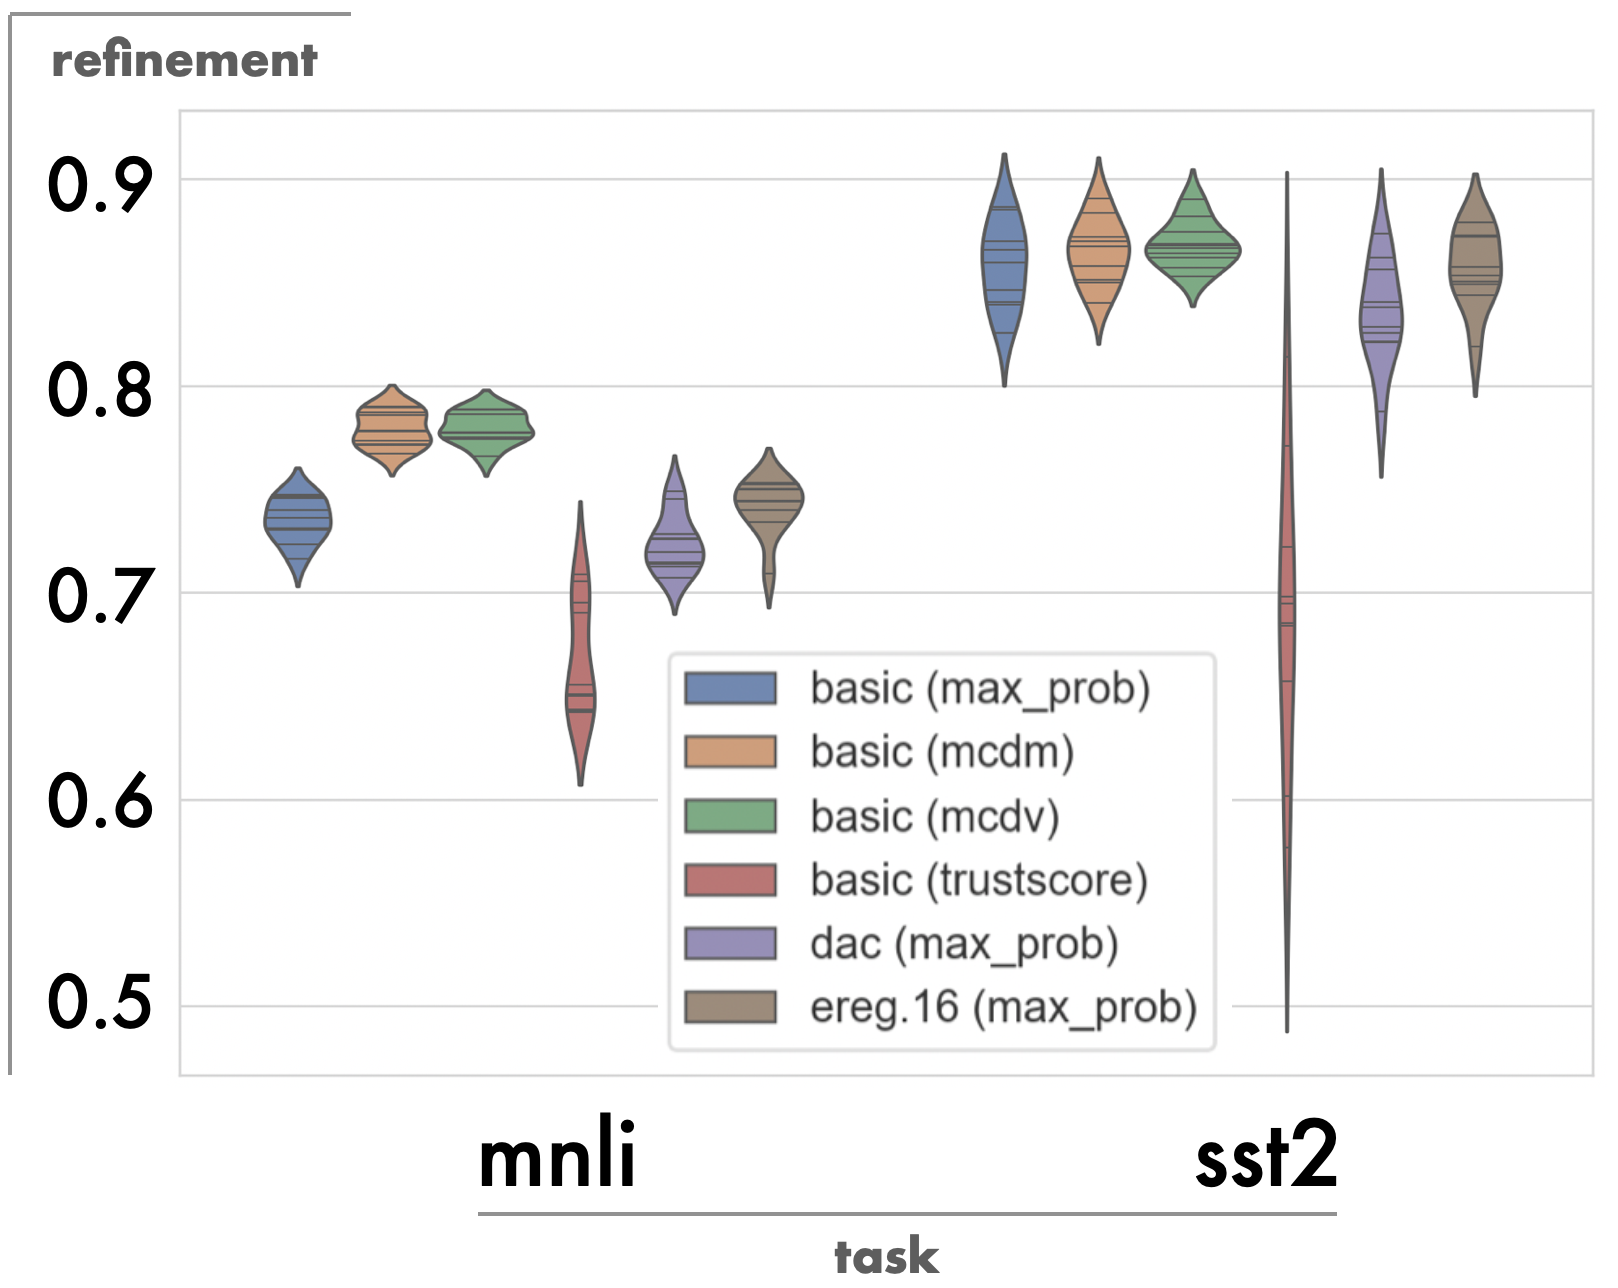
\includegraphics[width=0.48\textwidth]{violinplot2.png}
\caption{Results of several selective prediction techniques on two \textsc{GLUE} datasets. Each "string" of the violin corresponds to the refinement of a single trial on \textsc{GlueDev}, while the "body" of the violin is a kernel density estimation of the result distribution.}
\label{fig:posthocviolin}
\end{figure}

We quantify the phrase ``meaningfully better'' by estimating the likelihood that a candidate technique outperforms the basic \textsc{MaxProb} baseline. For a candidate technique $t$ and evaluation metric $m$, define random variable $X_{t,m}$ as the result of the following trial: 

\begin{itemize}
\item Choose a random task from a probability distribution $P_{task}$ over tasks.
\item Execute the candidate selective prediction technique $t$ and the baseline technique (i.e. \textsc{MaxProb}) and evaluate each using metric $m$ (e.g. refinement or \textsc{AUPR}).
\item If the candidate technique $t$ outperforms the baseline according to metric $m$, return 1. Otherwise, return 0.
\end{itemize}


\noindent The expected value $E(X_{t,m})$ tells us the likelihood that technique $t$ will outperform the baseline according to metric $m$ . Since we performed 10 trials for each of 6 GLUE tasks, we therefore have 60 samples\footnote{In this case, the task distribution $P_{task}$ is a uniform distribution over 6 GLUE tasks. Whether this is an effective proxy for NLP tasks in general is a fair question, but the community appears to have adopted GLUE as a useful benchmark.} for estimating $E(X_{t,m})$. Figure~\ref{fig:auprpointplot} shows the $E(X_{t,\mathsf{refinement}})$ estimate for eight techniques (including the random confidence baseline), along with a 95\% confidence interval. Somewhere between 62\% to 85\% of the time (with 95\% confidence), both \textsc{McdM} and \textsc{McdV} improve upon the \textsc{MaxProb} baseline according to refinement.  

On its own, refinement is sufficient to evaluate the techniques that only modify the confidence function (i.e. \textsc{McdM}, \textsc{McdV}, and \textsc{TrustScore}). Techniques that employ specialized loss functions, (e.g. error-regularization or DAC loss) should be evaluated using both refinement and AUPR, since these techniques might improve the efficiency of the confidence function while simultaneously sacrificing the quality of the prediction function. Simultaneous evaluation with AUPR and refinement allows us to distinguish whether improvements are achieved via enhancements to the confidence or the prediction function. In these experiments, AUPR and refinement largely agree about the quality of the loss specialization techniques, thus the techniques do not appear to impact the quality of the prediction function. In terms of improving the confidence function, \textsc{EReg} shows promise, but the trajectory of performance from minibatch size 8 to minibatch size 16 suggests that \textsc{EReg} needs a minibatch size of at least 32 to be a superior alternative to \textsc{MaxProb}.

\section{Related Work}

Selective prediction has a long tradition in machine learning, dating back to the  1950s \cite{chow1957optimum}. There is an extensive literature \cite{hellman1970nearest,fumera2002support,cortes2016learning} on training classifiers with the ability to abstain (also known as the "reject option"), usually specific to alternative classifiers like support vector machines.

There is also a significant literature \cite{platt1999probabilistic,guo2017calibration,kumar2018trainable,wang-etal-2020-inference,desai-durrett-2020-calibration} on the topic of \emph{calibration}, i.e. the development of probabilistically interpretable confidence measures. In this paper, we restrict our focus to the relative rankings of selective predictors, and not the confidence values themselves. 

\begin{figure}[tb]
\centering
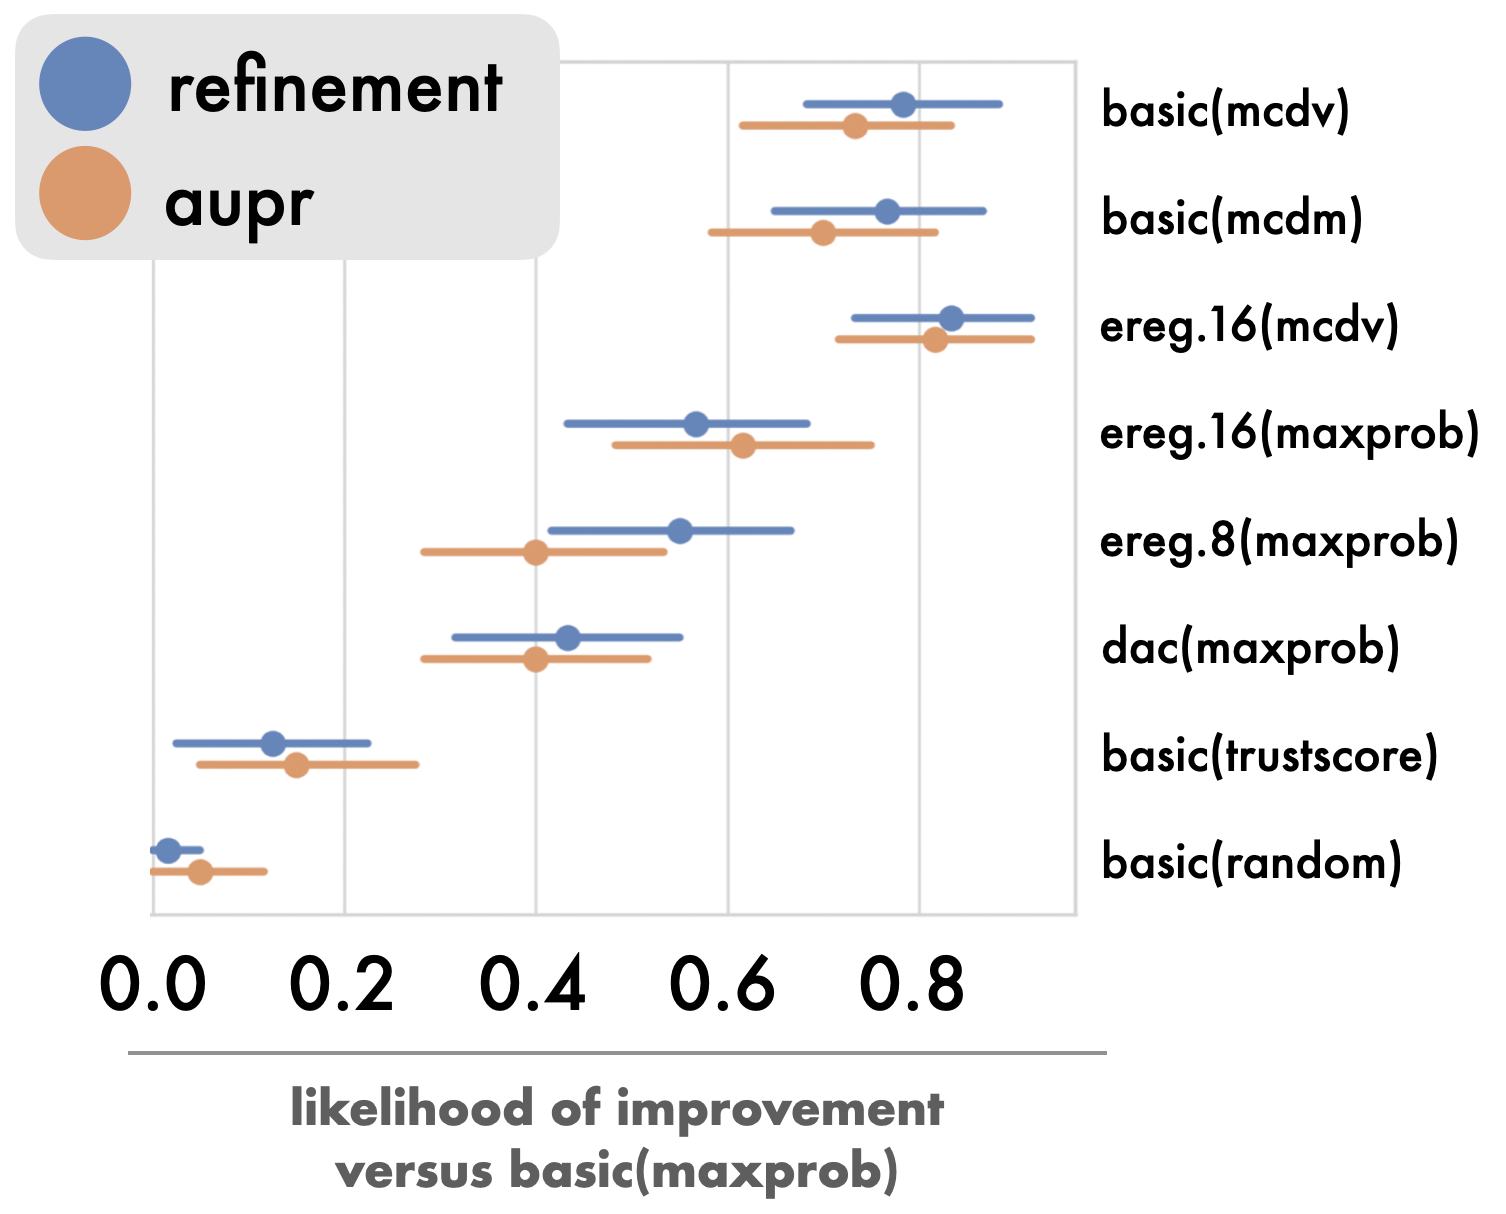
\includegraphics[width=0.48\textwidth]{pointplot2.png}
\caption{Estimate of the likelihood $E(X_{t,m})$ that technique $t$ outperforms the basic \textsc{MaxProb} baseline according to metric $m$ (refinement or \textsc{AUPR}). The bars show a 95\% confidence interval for this estimate.}\label{fig:auprpointplot}
\end{figure}

While our survey focuses on techniques designed to identify ambiguous instances in the evaluation set (and, for certain techniques, to also ignore label noise in the training set), there is also interest in selective prediction techniques that operate successfully under domain shift \cite{kamath-etal-2020-selective,liu2020energy}, i.e. when the distribution of evaluation instances differs from the training instances. Evaluation of such techniques is beyond the scope of the work described here, but we have plans to expand the \textsf{spred} package to evaluate selective prediction under domain shift.



\section{Conclusion}

We have provided a survey and empirical comparison of a diverse set of recent selective prediction techniques on a broad set of tasks. As a companion to the paper, the open-source Python package \textsf{spred} provides reproducible results and transparent methodology. Moreover, it comes with tutorials and unit tests that demonstrate how new techniques and tasks can be easily added. We hope this will facilitate novel selective prediction research on natural language domains.

\bibliography{anthology,custom}
\bibliographystyle{acl_natbib}

%\appendix

%\section{Hyperparameter Tuning Results}
%\label{sec:tuningappendix}

%Figure~\ref{fig:mcd_hparams}, Figure~\ref{fig:ts_hparams}, Figure~\ref{fig:ereg_hparams}, and Figure~\ref{fig:dac_hparams} show the experimental results for our hyperparameter tuning experiments. As with the final results, we visualize these using violin plots -- each ``string" of the violin corresponds to the result of a single trial.


%\begin{figure}[tb]
%\centering
%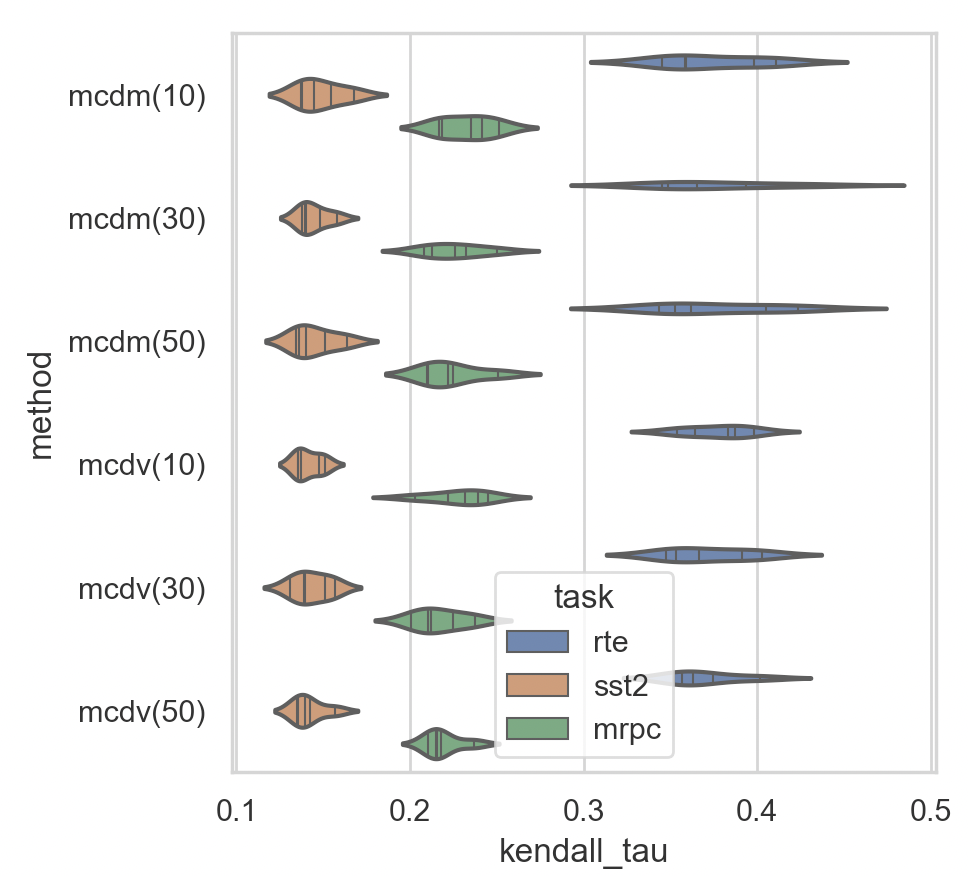
\includegraphics[width=0.48\textwidth]{mcd_hparams.png}
%\caption{Results of the hyperparameter tuning experiments for Monte Carlo Dropout.}
%\label{fig:mcd_hparams}
%\end{figure}

%\begin{figure}[p]
%\centering
%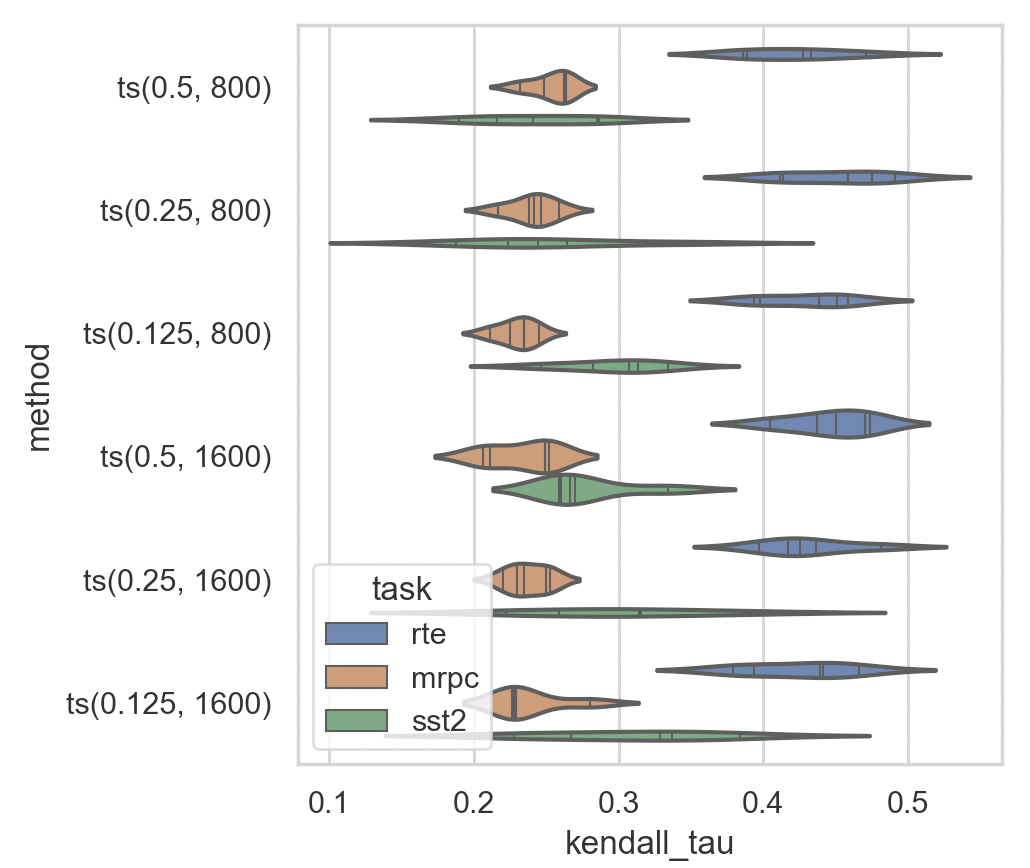
\includegraphics[width=0.48\textwidth]{ts_hparams.png}
%\caption{Results of the hyperparameter tuning experiments for TrustScore.}
%\label{fig:ts_hparams}
%\end{figure}

%\begin{figure}[p]
%\centering
%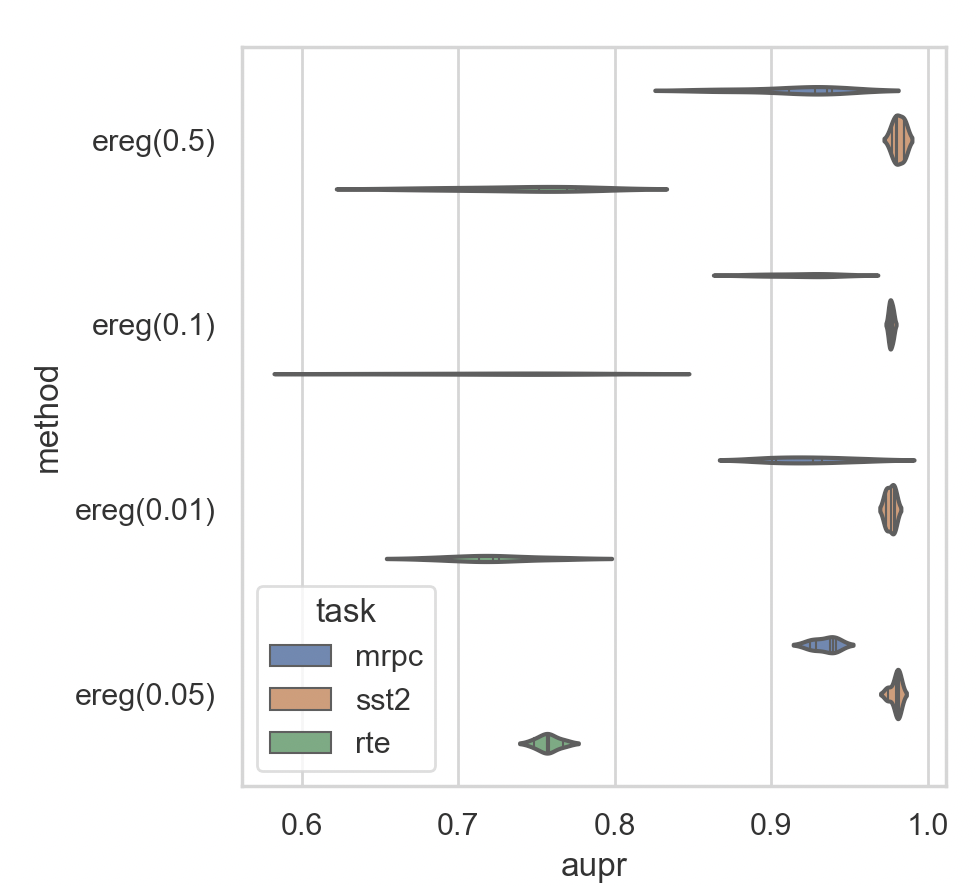
\includegraphics[width=0.48\textwidth]{ereg_hparams.png}
%\caption{Results of the hyperparameter tuning experiments for Error Regularization.}
%\label{fig:ereg_hparams}
%\end{figure}

%\begin{figure}[p]
%\centering
%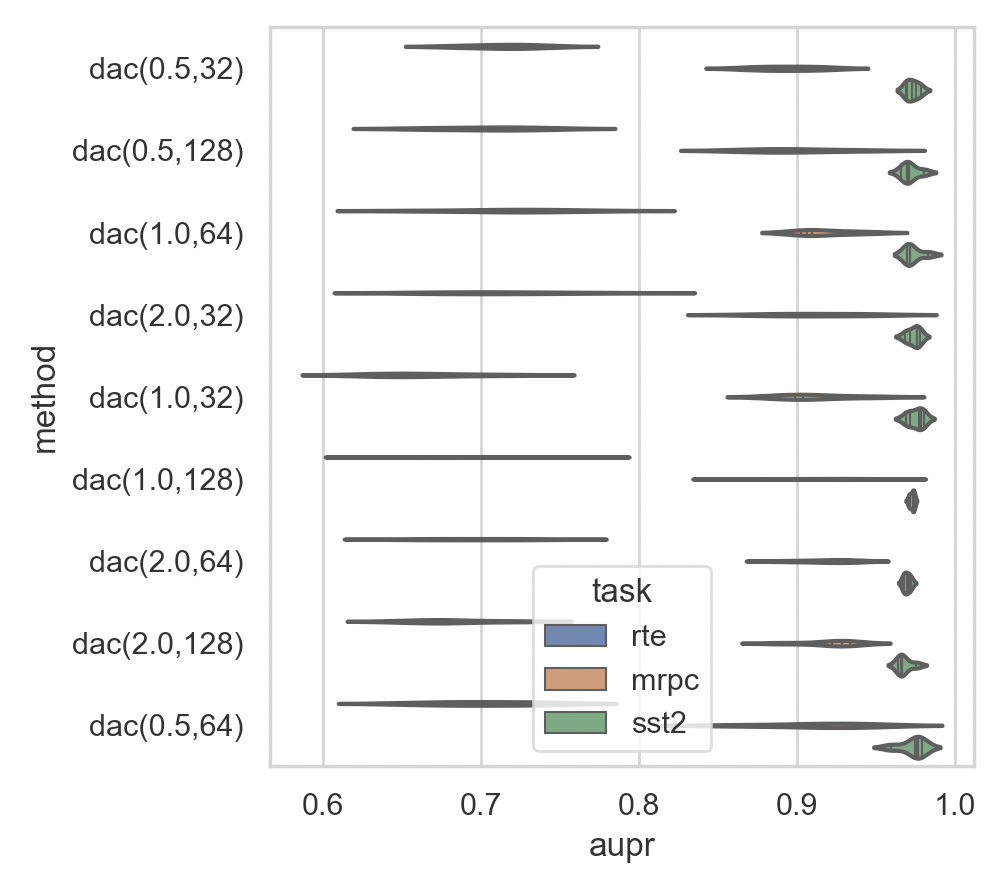
\includegraphics[width=0.48\textwidth]{dac_hparams.png}
%\caption{Results of the hyperparameter tuning experiments for the Deep Abstaining Classifier.}
%\label{fig:dac_hparams}
%\end{figure}


%\section{Machine Architecture and Running Time}

%The experiments were run on a single workstation with the following specifications:
%\begin{itemize}
%	\item \textbf{Operating System:} Ubuntu 20.04 	
%	\item \textbf{Processor:} AMD Threadripper 3990X: 64 cores, 2.90 GHz, 256 MB cache
%	\item \textbf{GPUs:} 2x RTX 3090
%	\item \textbf{Memory:} 256 GB
%	\item \textbf{Operating System Drive:} 2 TB SSD (NVMe)
%	\item \textbf{Data Drive:} 2 TB SSD (SATA)
%\end{itemize}

%\noindent To give the reader a sense of the relative cost of running each technique, we provide a representative result of a single trial on the above machine for the \textsc{RTE} task:

%\begin{itemize}
%	\item \textbf{Training time for basic BERT loss:} 201s
%	\item \textbf{Training time for BERT loss + error regularization:} 200s
%	\item \textbf{Training time for DAC loss:} 266s
%	\item \textbf{Evaluation time for \textsc{MaxProb}:} 1.72s
%	\item \textbf{Evaluation time for \textsc{McdM}/\textsc{McdV}:} 56s
%	\item \textbf{Evaluation time for \textsc{TrustScore}:} 40s
%\end{itemize}

\end{document}
